\documentclass[12pt,a4paper]{article}

% ==== Русский язык и кодировки (pdfLaTeX) ====
\usepackage[T2A]{fontenc}
\usepackage[utf8]{inputenc}
\usepackage[russian]{babel}

% ==== Геометрия ====
\usepackage{geometry}
\geometry{margin=2cm}

% ==== Встроенные шрифты TeX-дистрибутива ====

% ==== Внешний вид абзацев ====

% ==== Математика ====
\usepackage{amsmath, amssymb, amsthm}
\usepackage{eurosym}
\usepackage{etoolbox}

\renewcommand{\refname}{Список литературы}

\patchcmd{\thebibliography}
  {\section*{\refname}}
  {\section{\refname}}
  {}{}

\usepackage{booktabs}
\usepackage{longtable}
\usepackage{array}
\usepackage{xurl}

\newcommand{\RF}{RF}
\newcommand{\XGB}{XGB}
\newcommand{\feat}[1]{\path{#1}}

\numberwithin{equation}{section}
\usepackage{mathtools}
\newcommand{\xleftrightarrows}[2][]{%
  \overset{#2}{\underset{#1}{\rightleftarrows}}%
}

% ==== Графика/рисунки ====
\usepackage{graphicx}
\graphicspath{{images/}{outputs/figures/}}
\usepackage{float}
\usepackage[export]{adjustbox}

% ==== TikZ/PGFPlots ====
\usepackage{tikz}
\usetikzlibrary{arrows.meta,angles,quotes,calc}
\usepackage{pgfplots}
\pgfplotsset{compat=1.18}

% ==== Остальные пакеты ====
\usepackage{xcolor}
\usepackage{mdframed}
\usepackage{fancyhdr}
\usepackage{titlesec}
\usepackage{hyperref}
\usepackage[most]{tcolorbox}
\usepackage{enumitem}
\usepackage{cancel}
\usepackage{parskip}
\usepackage{listings}

% ==== Цвета ====
\definecolor{HSEblue}{HTML}{004C97}
\definecolor{HSElightblue}{HTML}{5B8CDE}
\definecolor{HSEdarkblue}{HTML}{00315E}

\definecolor{HSEgreen}{HTML}{007F5F}
\definecolor{HSElightgreen}{HTML}{00A47A}
\definecolor{HSEred}{HTML}{B80C09}
\definecolor{HSEorange}{HTML}{F26D00}
\definecolor{HSEpurple}{HTML}{6E56DB}
\definecolor{HSEteal}{HTML}{008B8B}
\definecolor{HSEgold}{HTML}{B8860B}
\definecolor{HSEmagenta}{HTML}{D63384}

\definecolor{HSEblack}{HTML}{000000}
\definecolor{HSEdarkgray}{HTML}{333333}
\definecolor{HSEgray}{HTML}{666666}
\definecolor{HSElightgray}{HTML}{999999}
\definecolor{HSEwhite}{HTML}{FFFFFF}

\definecolor{HSEbglight}{HTML}{F8F9FA}
\definecolor{HSEbglighter}{HTML}{F0F2F5}

% ==== Замены твоих "HSE-шрифтов" на стандартные переключатели ====
\newcommand{\thintext}[1]{{\mdseries #1}}
\newcommand{\blacktext}[1]{{\bfseries #1}}

% ==== Полезные обозначения из твоего исходника ====
\newcommand{\Od}[2]{O_{#1}\!\left(#2\right)}
\newcommand{\Odp}[2]{\dot O_{#1}\!\left(#2\right)}

% операторы (у babel/russian часто заняты \tg,\sh,\ch — освобождаем)
\let\sh\relax
\let\ch\relax
\DeclareMathOperator{\sgn}{sgn}
\DeclareMathOperator{\arcsh}{arcsh}
\DeclareMathOperator{\Lip}{Lip}
\renewcommand{\Re}{\operatorname{Re}}
\renewcommand{\Im}{\operatorname{Im}}
\providecommand{\NOD}{\operatorname{НОД}}
\providecommand{\NOK}{\operatorname{НОК}}

% множества функций (чтобы \UC, \Cont, \Bnd компилились)
\DeclareMathOperator{\UC}{UC}
\DeclareMathOperator{\Cont}{C}
\DeclareMathOperator{\Bnd}{Bnd}

% ==== Заголовки ====
\titleformat{\section}
  {\Large\bfseries\color{HSEblue}}
  {\thesection.}{0.5em}{}

\titleformat{\subsection}
  {\large\bfseries\color{HSEblue}}
  {\thesubsection.}{0.5em}{}

\titleformat{\subsubsection}
  {\normalsize\bfseries\color{HSEblue}}
  {\thesubsubsection.}{0.5em}{}

% ==== Колонтитулы ====
\pagestyle{fancy}
\fancyhf{}
\fancyhead[L]{\bfseries\nouppercase{\leftmark}}
\fancyhead[R]{\thepage}
\setlength{\headheight}{15pt}

\fancyfoot[C]{%
  Медведев Максим Юрьевич, Радько Роман Олегович
}
\renewcommand{\headrulewidth}{0.4pt}

% ==== Ссылки ====
\hypersetup{
  colorlinks=true,
  linkcolor=HSEblue,
  citecolor=HSEblue,
  urlcolor=HSEblue
}

% ==== tcolorbox базовый стиль ====
\newcommand{\sqbullet}{\raisebox{0.15ex}{\scalebox{0.4}{$\blacksquare$}}}

\tcbset{
  enhanced,
  breakable,
  boxrule=0.8pt,
  arc=6pt,
  boxsep=1.5pt,
  before upper=\par\vspace{6pt}\noindent,
  top=2pt,
  fonttitle=\bfseries,
  fontupper=\normalsize,
  attach boxed title to top left={yshift=-2mm},
  boxed title style={
    boxrule=0pt,
    frame hidden,
    interior style={fill opacity=1}
  }
}

% ===== Коробочки без нумерации (серый фон + нормальные отступы) =====

\tcbset{
  hsebox/.style={
    enhanced,
    breakable,
    boxrule=0.8pt,
    arc=6pt,
    boxsep=1.5pt,
    top=2pt,
    fonttitle=\bfseries,
    coltitle=white,
    attach boxed title to top left={yshift=-2mm,xshift=2mm},
    boxed title style={
      boxrule=0pt,
      frame hidden,
      interior style={fill opacity=1}
    },
    % ключевой зазор между заголовком и текстом (как "правильно")
    before upper=\par\vspace{6pt}\noindent\ignorespaces
  }
}

\newcommand{\DeclareHSEBox}[5]{%
  \newtcolorbox{#1}[2][]{%
    hsebox,
    colframe=#3,
    colback=HSEgray!10,          % <<< вернули серую заливку
    colbacktitle=#4,
    title={#2. ##2},
    before upper app={%
      \setlist[enumerate]{label=\color{#5}\arabic*., font=\color{#5}, itemsep=0.6em, topsep=0.3em}%
      \setlist[itemize]{label=\sqbullet, leftmargin=1.2em, itemsep=0.6em, topsep=0.3em}%
    },
    ##1
  }%
}

\DeclareHSEBox{definitionHSE}{Определение}{HSEblue}{HSEblue!90!black}{HSEblue}
\DeclareHSEBox{theoremHSE}{Теорема}{HSEgreen!70!black}{HSEgreen!80!black}{HSEgreen}
\DeclareHSEBox{lemmaHSE}{Лемма}{HSEteal!80!black}{HSEteal!85!black}{HSEteal}
\DeclareHSEBox{corollaryHSE}{Следствие}{HSEpurple!60!black}{HSEpurple!70!black}{HSEpurple}
\DeclareHSEBox{exampleHSE}{Пример}{HSEred!80!black}{HSEred!90!black}{HSEred}
\DeclareHSEBox{taskHSE}{Задача}{HSEmagenta!80!black}{HSEmagenta!90!black}{HSEmagenta}
\DeclareHSEBox{remarkHSE}{Замечание}{HSEorange!70!black}{HSEorange!80!black}{HSEorange}

% --- Доказательство ---
\renewenvironment{proof}[1][Доказательство]{\begin{center}\textbf{#1}\end{center}}{\hfill$\blacksquare$\par}

% === МЕТАДАННЫЕ ===
\title{\textbf{Прикладные задачи анализа данных}\\[0.3em]\large Анализ вклада внутренних и внешних признаков в качество прогнозирования спроса в розничной сети}
\author{Медведев Максим Юрьевич, Радько Роман Олегович --- БПМ255}

\begin{document}
\maketitle
\tableofcontents
\clearpage

\section{Введение}

\subsection{Постановка задачи}

Актуальность исследования обусловлена необходимостью повышения точности прогнозирования спроса в розничной торговле. Ошибки прогноза дневных продаж могут приводить к избыточным запасам, дефициту товаров и снижению эффективности операционного планирования.

Объектом исследования являются ежедневные продажи магазинов сети Rossmann. Предметом исследования выступает вклад внутренних и внешних признаков в качество прогнозирования продаж. При этом признаки продаж, строящиеся на основе прошлых значений целевой переменной из исходного датасета, рассматриваются как часть внутренних признаков.

Целью работы является оценка вклада дополнительных групп признаков в качество прогнозирования дневных продаж магазинов по сравнению с моделями, использующими базовый набор признаков датасета Rossmann Store Sales.

В рамках данной работы спрос отождествляется с фактическими продажами \texttt{Sales}, поскольку датасет не содержит данных о нереализованном спросе, то есть покупательский интерес, не завершившийся фактической продажей.

Для достижения поставленной цели решаются следующие задачи:
\begin{itemize}
    \item подготовка исходных данных и объединение их со справочной информацией о магазинах;
    \item формирование базового набора признаков и дополнительных групп признаков, включая исторические и внешние признаки;
    \item построение моделей для различных наборов признаков;
    \item сравнение качество моделей с использованием метрик;
    \item определение групп признаков, вносящих наибольший вклад в качество прогнозирования.
\end{itemize}

Исследовательская гипотеза состоит в том, что добавление внешних признаков может улучшить качество прогнозирования по сравнению с базовой моделью. В рамках этой гипотезы также оценивается, какие группы признаков дают наибольший вклад в снижение ошибки прогноза.

\subsection{Исходные данные}

В качестве исходных данных используется готовый набор Rossmann Store Sales, содержащий историческую информацию о продажах в 1115 магазинах немецкой сети дрогери \cite{kaggle2015rossmann}.

Представленные в датасете признаки можно классифицировать по типу данных следующим образом:
\begin{itemize}
    \item числовые;
    \item категориальные;
    \item бинарные;
    \item временные.
\end{itemize}

Таблица для обучения (\texttt{train.csv}) содержит следующие признаки:
\begin{itemize}
    \item \texttt{Store} — идентификатор магазина;
    \item \texttt{DayOfWeek} — день недели (временной признак);
    \item \texttt{Date} — дата (временной признак);
    \item \texttt{Sales} — дневная выручка (числовой признак), являющаяся целевой переменной задачи прогнозирования;
    \item \texttt{Customers} — число покупателей (числовой признак);
    \item \texttt{Open} — был ли магазин открыт (бинарный признак);
    \item \texttt{Promo} — была ли в этот день акция (бинарный признак);
    \item \texttt{StateHoliday} — тип государственного праздника или его отсутствие (категориальный признак);
    \item \texttt{SchoolHoliday} — школьные каникулы (бинарный признак).
\end{itemize}
Признак \texttt{Customers} не использовался при обучении моделей, поскольку в реальной задаче прогнозирования будущих продаж количество покупателей заранее неизвестно. Использование этого признака могло бы привести к утечке информации, то есть к ситуации, когда модель получает данные, которые в реальной задаче заранее были бы неизвестны.

\texttt{test.csv} содержит наблюдения, для которых необходимо спрогнозировать целевую переменную \texttt{Sales}. В настоящем исследовании этот файл не использовался, поскольку в нём отсутствуют фактические значения \texttt{Sales}, необходимые для расчёта метрик качества. Поэтому оценка моделей проводилась на валидационной выборке, сформированной с помощью временного разделения данных из \texttt{train.csv}.

Таблица \texttt{store.csv} содержит справочную информацию по магазинам:
\begin{itemize}
    \item \texttt{Store} — идентификатор магазина;
    \item \texttt{StoreType} — тип магазина (категориальный признак);
    \item \texttt{Assortment} — тип ассортимента (категориальный признак);
    \item \texttt{CompetitionDistance} — расстояние до ближайшего конкурента (числовой признак);
    \item \texttt{CompetitionOpenSinceMonth} — месяц, когда ближайший конкурент начал работать (временной признак);
    \item \texttt{CompetitionOpenSinceYear} — год, когда ближайший конкурент начал работать (временной признак);
    \item \texttt{Promo2} — участвует ли магазин в длительной повторяющейся промо-кампании (бинарный признак);
    \item \texttt{Promo2SinceWeek} — неделя, с которой началась \texttt{Promo2} (временной признак);
    \item \texttt{Promo2SinceYear} — год начала Promo2 (временной признак);
    \item \texttt{PromoInterval} — месяцы проведения длительной промо-кампании \texttt{Promo2} (категориальный признак).
\end{itemize}

Также использовалась таблица \texttt{store\_states.csv}, содержащая соответствие магазинов федеральным землям Германии. Она применялась для объединения данных о магазинах с внешними признаками, зависящими от региона.

\section{Обзор литературы}

Прогнозирование спроса в розничной торговле является сложной задачей, поскольку объём продаж формируется под влиянием множества факторов, включая календарные периоды, характеристики магазина, промоакции, сезонность и условия внешней среды, например погоду. В обзоре Р.~Филдса, Ш.~Ма и С.~Колассы отмечается, что прогнозирование розничного спроса важно как для долгосрочного управления компанией, так и для ежедневных решений на уровне отдельных магазинов и товаров \cite{fildes2022retail}.

В современных исследованиях и соревнованиях по прогнозированию спроса широко применяются методы машинного обучения для табличных данных, включая ансамблевые модели на основе решающих деревьев. Результаты соревнования M5 показывают, что в задачах розничного прогнозирования важную роль играют признаки, основанные на прошлых значениях продаж, а также календарные факторы и информация о промоактивности \cite{makridakis2022m5}. Отдельные исследования также подчёркивают значимость конструирования промо-признаков. Так, Ш.~Ма, Р.~Филдс и Т.~Хуанг рассматривают задачу прогнозирования продаж на уровне SKU с учётом большого числа признаков, позволяющих учитывать влияние промоакций не только на отдельный товар, но и на связанные с ним товары \cite{ma2016demand}.

Связь погодных условий с продажами также рассматривается в прикладных исследованиях розничной торговли. Например, Н.~Роуз и Л.~Долега анализируют связь между погодными условиями и ежедневными продажами крупного ритейлера, используя, в том числе, методы случайного леса \cite{rose2022weather}. Результаты их работы позволяют предположить, что погодные признаки могут быть полезны для прогнозирования спроса.

Отдельное направление исследований связано с использованием поискового интереса как внешнего индикатора потребительского спроса. Х.~Чой и Х.~Вэриан показали, что данные Google Trends могут быть полезны для краткосрочного прогнозирования экономической активности, поскольку поисковые запросы отражают текущий интерес пользователей до публикации официальной статистики \cite{choi2012predicting}. В рамках данной работы это служит основанием для включения признака \texttt{GoogleTrend} в экспериментальный анализ.

Таким образом, существующие исследования подтверждают целесообразность проверки внешних признаков в задачах прогнозирования спроса. При этом заранее нельзя утверждать, что каждый внешний источник данных улучшит качество модели. Его вклад зависит от временного горизонта прогноза, качества агрегации данных, типа товаров и уже имеющихся внутренних признаков. Для оценки моделей временных рядов также важно учитывать порядок наблюдений. В литературе по прогнозированию для этого применяются разбиения, имитирующие прогнозирование будущих периодов, например схема последовательного смещения точки прогноза (rolling forecasting origin) \cite{hyndman2021fpp}; в данной работе использовалось более простое одно временное разбиение на обучающую и валидационную выборки.

\section{Методы}

\subsection{Общая схема}

После анализа структуры исходных данных задача была сформулирована как \textbf{задача регрессии}: на основе доступных характеристик наблюдения необходимо предсказать дневной объём продаж \texttt{Sales}. Поскольку данные представлены в виде временного ряда, при построении и оценке моделей важно сохранять хронологический порядок наблюдений и не перемешивать обучающую и валидационную выборки случайным образом.

В качестве основного направления решения были выбраны методы машинного обучения для табличных данных, в первую очередь ансамблевые методы на основе решающих деревьев. Такой выбор обусловлен тем, что продажи в розничной торговле могут зависеть от большого числа разнородных признаков, а связь между этими признаками и целевой переменной может быть нелинейной.

Одним из наиболее подходящих методов для такой постановки является градиентный бустинг над решающими деревьями. Метод градиентного бустинга был формализован в работе Дж.~Фридмана, где рассматривается как последовательное построение аддитивной модели, минимизирующей функцию потерь \cite{friedman2001greedy}. В практической части работы использовалась реализация XGBoost, предложенная Т.~Ченом и К.~Гестрином \cite{chen2016xgboost}. Данный алгоритм хорошо подходит для задач с большим числом наблюдений и неоднородными признаками, что соответствует структуре рассматриваемого набора данных.

Также в качестве альтернативных моделей были рассмотрены линейная регрессия и случайный лес. Линейная регрессия использовалась в качестве базовой интерпретируемой модели, с которой сравнивались более сложные алгоритмы машинного обучения. Метод случайного леса был систематически описан Л.~Брейманом \cite{breiman2001random}. В данной работе он используется как альтернативный ансамблевый метод, поскольку способен учитывать нелинейные зависимости между признаками без последовательного построения деревьев, характерного для бустинга.

Выбор ансамблевых моделей на основе решающих деревьев и лаговых признаков соответствует подходам, широко применяемым в современных задачах прогнозирования розничных продаж. В частности, результаты соревнования M5 показывают значимость моделей градиентного бустинга и признаков, основанных на прошлых значениях продаж \cite{makridakis2022m5}.

Общий ход исследования был следующим. Сначала исходные данные были очищены и объединены со справочной информацией о магазинах. Затем были сформированы дополнительные признаки: календарные признаки, фиктивные признаки для категориальных признаков, признаки праздников, погодные признаки, признак уровня безработицы, Google Trends, взаимодействия промо-акций и погоды, а также лаговые признаки продаж. Далее все признаки были разделены на несколько смысловых групп, что позволило провести серию экспериментов с различными наборами признаков.

Для оценки качества моделей исходная обучающая выборка была разделена на обучающую и валидационную части по времени. Наблюдения до \texttt{2015-06-01} использовались для обучения, а наблюдения начиная с \texttt{2015-06-01} --- для валидации.

Качество моделей оценивалось с помощью трёх метрик: RMSPE, MAE и $R^2$. Основной метрикой сравнения была выбрана RMSPE, поскольку она измеряет относительную ошибку прогноза и учитывает различия в масштабе продаж между магазинами. После сравнения моделей и вариантов признаков для лучших моделей был проведён анализ важности признаков, позволяющий определить, какие признаки были наиболее важны для формирования прогноза.

\subsection{Организация проекта и воспроизводимость экспериментов}

Для обеспечения воспроизводимости экспериментов проект был организован следующим образом:

\begin{verbatim}
Sem/
|-- data/
|   |-- raw/
|   |-- external/
|   `-- cache/
|-- src/
|   |-- data/
|   `-- models/
|-- outputs/
|   |-- figures/
|   |-- models/
|   `-- reports/
|-- notebooks/
|-- requirements.txt
`-- README.md
\end{verbatim}

В папке \texttt{data/raw/} хранятся исходные данные Rossmann:
\begin{itemize}
    \item \texttt{train.csv},
    \item \texttt{test.csv},
    \item \texttt{store.csv},
    \item \texttt{store\_states.csv}.
\end{itemize}

В папке \texttt{data/external/} хранятся внешние данные:
\begin{itemize}
    \item \texttt{weather\_daytime.csv},
    \item \texttt{googletrend\_self.csv},
    \item \texttt{unemployment\_germany.csv}.
\end{itemize}

Погодные данные были получены из исторического архива Open-Meteo \cite{openmeteo} для столиц федеральных земель Германии. Для каждой федеральной земли загружались почасовые значения температуры воздуха, количества осадков и продолжительности солнечного сияния. Далее были оставлены только наблюдения за часы работы магазинов с 9:00 до 20:00, после чего данные агрегировались до дневного уровня. В результате были сформированы четыре погодных признака: \texttt{temperature\_mean} --- средняя температура за рабочие часы, \texttt{temperature\_max} --- максимальная температура за рабочие часы, \texttt{precipitation\_sum} --- сумма осадков за рабочие часы, \texttt{sunshine\_sum} --- суммарная продолжительность солнечного сияния за рабочие часы.

Данные Google Trends \cite{googletrends} были сформированы для запроса \texttt{rossmann} по федеральным землям Германии. Индекс Google Trends представляет собой относительный нормированный показатель поискового интереса в диапазоне от 0 до 100, где 100 соответствует максимальному уровню интереса в выбранном периоде и регионе; в использованной выгрузке он имел недельную частоту. В данной версии предобработки недельные значения присоединялись к дневным данным по совпадающим датам и регионам, а отсутствующие значения далее заполнялись нулями вместе с остальными пропусками. Поэтому результаты для группы \texttt{google\_trends} интерпретировались осторожно.

Показатель безработицы был получен из FRED \cite{fredunemployment} как месячный показатель Harmonized Unemployment Rate для Германии. Внешние данные объединялись с основным датасетом по дате и региону; для месячного показателя безработицы значение месяца распространялось на все дни соответствующего месяца.

В папке \texttt{src/models/} находятся скрипты обучения и оценки моделей:
\begin{itemize}
    \item \texttt{common.py} --- содержит общие функции подготовки данных, формирования признаков и расчёта метрик;
    \item \texttt{model\_runtime.py} --- содержит вспомогательные функции для сохранения моделей, конфигураций и метаданных экспериментов;
    \item \texttt{baselines.py} --- рассчитывает наивные и простые базовые прогнозы для сравнения с моделями машинного обучения;
    \item \texttt{feature\_variant\_search.py} --- перебирает варианты признаков и обучает модели на разных наборах;
    \item \texttt{linear\_regression.py} --- обучает модель линейной регрессии на выбранном наборе признаков и сохраняет результаты;
    \item \texttt{random\_forest.py} --- обучает модель случайного леса на выбранном наборе признаков и строит график важности признаков;
    \item \texttt{xgboost\_shap.py} --- обучает модель XGBoost на выбранном наборе признаков и выполняет SHAP-анализ важности признаков.
\end{itemize}

В папке \texttt{outputs/models/} сохраняются обученные модели и метаданные:
\begin{itemize}
    \item \texttt{linear\_regression.pkl},
    \item \texttt{random\_forest.pkl},
    \item \texttt{xgboost\_shap\_holidays\_lags.json},
    \item \texttt{feature\_columns.json},
    \item \texttt{preprocessing\_config.json}.
\end{itemize}

В папке \texttt{outputs/reports/} сохраняются результаты экспериментов:
\begin{itemize}
    \item \texttt{baseline\_metrics.csv},
    \item \texttt{baseline\_metrics.json},
    \item \texttt{feature\_variant\_metrics.csv},
    \item \texttt{feature\_variant\_metrics.json},
    \item \texttt{feature\_importance\_xgboost.csv},
    \item \texttt{experiments\_summary.md}.
\end{itemize}

В папке \texttt{src/data/} находятся скрипты подготовки внешних данных:
\begin{itemize}
    \item \texttt{weather.py},
    \item \texttt{google\_trends\_parsing.py},
    \item \texttt{unemployment.py}.
\end{itemize}

Актуальная версия проекта размещена в открытом репозитории GitHub:
\url{https://github.com/alwaysnervous/rossman}.

Репозиторий содержит исходный код предобработки данных, обучения моделей,
проведения экспериментов, построения графиков, а также итоговый отчёт,
результаты экспериментов и файл \texttt{requirements.txt} с используемыми
зависимостями. Наличие репозитория позволяет проследить структуру проекта и
воспроизвести основные этапы исследования. Бинарные файлы обученных моделей и
служебные файлы окружения не включались в репозиторий, поскольку они не
являются необходимыми для анализа структуры проекта и могут быть заново
получены запуском соответствующих скриптов.

\subsection{Постановка экспериментов}

Во всех экспериментах использовался датасет Rossmann с целевой переменной \texttt{Sales}.

Из обучающей выборки были исключены строки, соответствующие дням, когда магазин был закрыт: \(\texttt{Open} = 0\). Такие наблюдения не отражают фактический потребительский спрос, поскольку продажи в эти дни равны нулю. Поэтому в дальнейшем задача рассматривается как прогнозирование продаж для дней, когда магазин открыт. После такой фильтрации признак \texttt{Open} фактически становится константным и не используется при интерпретации результатов как содержательный признак.

Разделение на обучающую и валидационную выборки выполнялось по времени:

\begin{itemize}
    \item обучающая выборка: даты до \texttt{2015-06-01};
    \item валидационная выборка: даты начиная с \texttt{2015-06-01}.
\end{itemize}

Категориальные признаки \texttt{StateHoliday}, \texttt{StoreType}, \texttt{Assortment} и \texttt{PromoInterval} кодировались методом прямого кодирования категориальных признаков (one-hot encoding). При кодировании использовался параметр \texttt{dummy\_na=True}, поэтому для пропущенных значений создавался отдельный фиктивный признак.

После кодирования категориальных признаков оставшиеся пропуски в числовых признаках заполнялись нулём: \(\texttt{fillna(0)}\). В данной работе это значение использовалось как техническое обозначение отсутствующей или неизвестной информации.

\subsubsection{Формирование лаговых признаков и контроль утечки данных}

Отдельное внимание было уделено лаговым признакам продаж, поскольку они позволяют учитывать зависимость текущего объёма продаж от предыдущих значений и отражать динамику спроса. Для каждого магазина лаговые признаки вычислялись внутри соответствующего временного ряда после сортировки наблюдений по \texttt{Store} и \texttt{Date}. Поскольку строки с закрытыми магазинами были исключены, индекс \(t\) в формулах ниже обозначает номер доступного наблюдения для конкретного магазина, а не обязательно соответствующий календарный день. При расчёте использовались только значения продаж, предшествующие текущему наблюдению:
\[
\texttt{Sales\_Lag1}_{s,t} = \texttt{Sales}_{s,t-1},
\]
\[
\texttt{Sales\_Lag7}_{s,t} = \texttt{Sales}_{s,t-7},
\]
\[
\texttt{Sales\_Rolling7}_{s,t} =
\frac{1}{m_{s,t}}\sum_{k=1}^{m_{s,t}}\texttt{Sales}_{s,t-k},
\quad m_{s,t}=\min(7,t-1).
\]

Здесь \(s\) обозначает магазин, а \(t\) --- порядковый номер доступного наблюдения для данного магазина. Таким образом, \texttt{Sales\_Lag1} соответствует предыдущему доступному наблюдению, а \texttt{Sales\_Lag7} --- седьмому предыдущему доступному наблюдению. При формировании признаков не использовались значения продаж за текущий день и будущие наблюдения. Эксперимент соответствует прогнозированию на один шаг вперёд (one-step-ahead forecasting): при прогнозировании очередного дня предполагается, что фактические продажи за предыдущие доступные дни уже известны. Для прогноза на несколько дней без обновления фактических продаж потребовалась бы отдельная рекурсивная схема расчёта лаговых признаков.

Следует также отметить, что признаки \texttt{DayOfWeek} и \texttt{dayofweek} содержательно описывают одно и то же. Первый признак присутствует в исходном датасете Rossmann, а второй был автоматически извлечён из поля \texttt{Date} средствами \texttt{pandas}. Они отличаются кодировкой: \texttt{DayOfWeek} принимает значения от 1 до 7, тогда как \texttt{dayofweek} --- от 0 до 6. Поэтому при интерпретации важности признаков их следует рассматривать совместно как признаки дня недели. В более строгой версии предобработки один из этих признаков следовало бы исключить, чтобы уменьшить избыточность признакового пространства.

Признак \texttt{Store} использовался как идентификатор магазина, поэтому не интерпретировался как обычный числовой признак.

\subsection{Метрики качества}
Для оценки качества прогнозирования использовались три метрики: RMSPE, MAE и коэффициент детерминации \(R^2\).

Пусть \(y_i\) обозначает фактическое значение продаж, \(\hat{y}_i\) --- прогноз модели, \(\bar{y}\) --- среднее фактическое значение целевой переменной, а \(n\) --- число наблюдений.

Основной метрикой сравнения была выбрана RMSPE:
\[
\mathrm{RMSPE} = \sqrt{\frac{1}{n}\sum_{i=1}^{n}\left(\frac{y_i - \hat{y}_i}{y_i}\right)^2}.
\]
Данная метрика измеряет относительную ошибку прогноза и поэтому подходит для сравнения магазинов с различным масштабом продаж.

При расчёте RMSPE учитывались только наблюдения с положительным фактическим значением продаж, поскольку метрика содержит деление на фактическое значение целевой переменной.

Дополнительно использовалась средняя абсолютная ошибка MAE:
\[
\mathrm{MAE} = \frac{1}{n}\sum_{i=1}^{n}|y_i - \hat{y}_i|.
\]
MAE показывает среднюю абсолютную ошибку прогноза в денежных единицах и является удобной для практической интерпретации.

Также рассчитывался коэффициент детерминации:
\[
R^2 = 1 - \frac{\sum_{i=1}^{n}(y_i - \hat{y}_i)^2}{\sum_{i=1}^{n}(y_i - \bar{y})^2}.
\]
Метрика \(R^2\) показывает долю вариации целевой переменной, объясняемую моделью, и использовалась как вспомогательный показатель качества.

\subsection{Гиперпараметры моделей}

Для модели XGBoost использовались следующие параметры:
\begin{itemize}
    \item \texttt{max\_depth = 5}

    Ограничивает максимальную глубину каждого дерева. Чем больше глубина, тем более сложные зависимости может учитывать модель, однако при слишком большом значении возрастает риск переобучения. В работе было выбрано оптимальное значение \texttt{max\_depth = 5}.
    \item \texttt{learning\_rate = 0.05}

    Задаёт вклад каждого нового дерева в итоговый прогноз. Малое значение \feat{learning_rate} делает обучение более плавным, что снижает риск переобучения, но требует большего числа boosting-итераций.
    \item \texttt{objective = reg:squarederror}

    Задаёт функцию потерь для задачи регрессии.
    \item \texttt{eval\_metric = rmse}

    Указывает, что во время обучения качество модели на обучающей и валидационной выборках отслеживалось по RMSE.
    \item \texttt{num\_boost\_round = 3000}

    Задаёт максимальное число boosting-итераций, то есть максимальное количество деревьев, которые может построить модель. Это верхняя граница, а не обязательно фактическое число использованных деревьев.
    \item \texttt{early\_stopping\_rounds = 50}

    Задаёт число итераций без улучшения качества на валидационной выборке, после которого обучение останавливается.
    \item \texttt{seed = 42}

    Фиксирует генератор случайных чисел, что позволяет при повторном запуске эксперимента с теми же данными, параметрами и версиями библиотек получать одинаковые результаты обучения.
\end{itemize}

Номер лучшей итерации при использовании early stopping сохранялся в служебном JSON-файле, однако в основную таблицу результатов он не включался, так как не является метрикой качества и неприменим к Random Forest.

Для модели Random Forest использовались параметры:
\begin{itemize}
    \item \texttt{n\_estimators = 100}
    
    Задаёт количество деревьев в ансамбле. Большее число деревьев обычно повышает устойчивость модели и снижает разброс прогнозов, но увеличивает время обучения и размер модели.
    \item \texttt{max\_depth = 15}

    Ограничивает глубину деревьев. Это контролирует сложность модели и снижает риск переобучения. В отличие от XGBoost, в Random Forest деревья обучаются независимо, а случайность задаётся bootstrap-подвыборками наблюдений и случайным выбором признаков при разбиениях.

    \item \texttt{random\_state = 42}

    Аналогично \texttt{seed} в XGBoost.
    \item \texttt{n\_jobs = -1}

    Означает использование всех доступных ядер процессора для параллельного обучения деревьев. Этот параметр влияет на скорость обучения, но не является параметром качества модели.
\end{itemize}

\section{Результаты}

\subsection{Сравнение моделей и вариантов признаков}

Был выполнен перебор всех комбинаций групп признаков для трёх моделей: Linear Regression, Random Forest и XGBoost.

Во всех экспериментах использовался базовый набор признаков (\texttt{base}), включающий используемые исходные признаки из \texttt{train.csv} и \texttt{store.csv}, а также календарные признаки и фиктивные признаки, полученные методом прямого кодирования категориальных признаков (one-hot encoding):

\begin{itemize}
    \item идентификатор магазина:
    
    \texttt{Store};

    \item исходные календарные и бинарные признаки из \texttt{train.csv}:
    
    \texttt{DayOfWeek},
    \texttt{Open},
    \texttt{Promo},
    \texttt{SchoolHoliday};

    \item признаки конкуренции и промо-акций из \texttt{store.csv}:
    
    \begin{tabular}{@{}l@{}}
    \texttt{CompetitionDistance},\\
    \texttt{CompetitionOpenSinceMonth},\\
    \texttt{CompetitionOpenSinceYear},\\
    \texttt{Promo2},\\
    \texttt{Promo2SinceWeek},\\
    \texttt{Promo2SinceYear};
    \end{tabular}

    \item календарные признаки, извлечённые из \texttt{Date}:
    
    \texttt{year},
    \texttt{month},
    \texttt{day},
    \texttt{dayofweek},
    \texttt{WeekOfYear},
    \texttt{IsMonthEnd},
    \texttt{IsFriday};

    \item фиктивные признаки для категориальных признаков:
    
    \begin{tabular}{@{}l@{}}
    \texttt{StateHoliday\_0}, \texttt{StateHoliday\_a},\\
    \texttt{StateHoliday\_b}, \texttt{StateHoliday\_c},\\
    \texttt{StateHoliday\_nan},
    \end{tabular}
    
    \texttt{StoreType\_a},
    \texttt{StoreType\_b},
    \texttt{StoreType\_c},
    \texttt{StoreType\_d},
    \texttt{StoreType\_nan},
    
    \texttt{Assortment\_a},
    \texttt{Assortment\_b},
    \texttt{Assortment\_c},
    \texttt{Assortment\_nan},
    
    \texttt{PromoInterval\_Jan,Apr,Jul,Oct},
    
    \texttt{PromoInterval\_Feb,May,Aug,Nov},
    
    \texttt{PromoInterval\_Mar,Jun,Sept,Dec},
    
    \texttt{PromoInterval\_nan}.
\end{itemize}

В данной работе исторические признаки продаж рассматриваются как внутренние, поскольку они строятся на основе прошлых значений \texttt{Sales}. Под историческими признаками продаж далее понимаются лаговые признаки \texttt{Sales\_Lag1}, \texttt{Sales\_Lag7} и один признак скользящего среднего \texttt{Sales\_Rolling7}.

Погодные данные, Google Trends и уровень безработицы относятся к внешним признакам, поскольку были получены из дополнительных источников, не входящих в исходные таблицы Rossmann. Праздничные признаки \texttt{PublicHoliday}, \texttt{BeforeHoliday} и \texttt{AfterHoliday} также были сформированы отдельно, поэтому они не объединяются с исходными признаками \texttt{StateHoliday} и \texttt{SchoolHoliday}.

Дополнительно перебирались следующие 6 групп признаков:
\begin{itemize}
    \item погодные признаки (\texttt{weather}):
    
    \texttt{temperature\_mean},
    \texttt{temperature\_max},
    \texttt{precipitation\_sum},
    \texttt{sunshine\_sum};

    производные погодные признаки:
    
    \texttt{TempRange},
    \texttt{IsRainy},
    \texttt{IsSunny},
    \texttt{IsHot},
    \texttt{IsCold};

    \item Google Trends (\texttt{google\_trends}):
    
    \texttt{GoogleTrend};

    \item уровень безработицы (\texttt{unemployment}):
    
    \texttt{UnemploymentRate};

    \item праздники (\texttt{holidays}):
    
    \texttt{PublicHoliday},
    \texttt{BeforeHoliday},
    \texttt{AfterHoliday};

    \item взаимодействия промо и погоды (\(\texttt{promo\_weather}\)):
    
    \texttt{Promo\_Temperature},
    \texttt{Promo\_Sunny},
    \texttt{Promo\_Rainy};
	
	Данные признаки были рассчитаны как произведение признака наличия промо-акции
\texttt{Promo} на соответствующие погодные признаки:
\[
\texttt{Promo\_Temperature} = \texttt{Promo} \cdot \texttt{temperature\_mean},
\]
\[
\texttt{Promo\_Sunny} = \texttt{Promo} \cdot \texttt{IsSunny},
\]
\[
\texttt{Promo\_Rainy} = \texttt{Promo} \cdot \texttt{IsRainy}.
\]

    \item лаговые признаки продаж (\texttt{lags}):
    
    \texttt{Sales\_Lag1},
    \texttt{Sales\_Lag7},
    \texttt{Sales\_Rolling7}.
\end{itemize}

Теоретически это даёт $2^6 = 64$ комбинаций, однако группа взаимодействий промо и погоды вычисляется через погодные признаки. Поэтому комбинации, где
\texttt{promo\_weather = true}, но \texttt{weather = false}, были исключены.

Итоговое число вариантов признаков составило \(64-2^4=64-16=48\). Для каждого варианта были
обучены три модели: Linear Regression, Random Forest и XGBoost. Таким образом, всего было проведено
$48 \times 3 = 144$ эксперимента.

Варианты признаков были отсортированы по \(\mathrm{RMSPE}\), так как эта метрика отражает относительную ошибку прогноза и лучше подходит для сравнения качества моделей при разных уровнях продаж.

Например, если магазин имеет средний уровень продаж в \(1\ 000\EUR\), то ошибка в \(500\EUR\) будет более существенной, тогда как для магазина со средним уровнем продаж в \(20\ 000\EUR\) такая же абсолютная ошибка будет иметь меньший относительный масштаб. Поэтому метрика \(\mathrm{MAE}\), несмотря на удобную интерпретацию в евро, не была использована в качестве основной метрики ранжирования.

Метрика \(R^2\) также не была выбрана в качестве основного критерия, поскольку она показывает долю вариации целевой переменной, объясняемую моделью, но не измеряет напрямую относительный размер ошибки прогноза. Иными словами, \(R^2\) сравнивает ошибку модели с общим разбросом фактических значений относительно среднего, а не оценивает ошибку относительно каждого конкретного значения продаж. Поэтому при прогнозировании продаж, где наблюдения могут существенно различаться по масштабу, \(R^2\) использовалась только как вспомогательная метрика.

\subsubsection{Базовые прогнозы}

Помимо моделей машинного обучения были рассчитаны простые базовые прогнозы, характерные для задач прогнозирования временных рядов. В качестве наивных прогнозов использовались продажи того же магазина из предыдущего доступного наблюдения и из седьмого предыдущего доступного наблюдения. Дополнительно были рассчитаны более содержательные агрегированные базовые прогнозы: средние продажи по магазину и средние продажи по паре магазин -- день недели. Все средние значения рассчитывались только на обучающей выборке. Результаты приведены в таблице~\ref{tab:naive_baselines}.

\begin{table}[H]
\centering
\caption{Качество базовых прогнозов}
\label{tab:naive_baselines}
\begin{tabular}{l r r r}
\toprule
Модель & RMSPE & MAE & $R^2$ \\
\midrule
Среднее по магазину и дню недели & 0.2271 & 1276 & 0.7073 \\
Naive Lag-1 & 0.3094 & 1364 & 0.5445 \\
Среднее по магазину & 0.3177 & 1487 & 0.5952 \\
Naive Lag-7 & 0.4793 & 2434 & 0.0307 \\
\bottomrule
\end{tabular}
\end{table}

Сравнение показывает, что лучшие модели машинного обучения существенно превосходят базовые прогнозы по RMSPE. Наиболее сильным среди простых базовых вариантов оказался прогноз на основе средних продаж по магазину и дню недели, однако его RMSPE равна \(0.2271\), что заметно хуже результатов Random Forest и XGBoost. Это подтверждает, что для повышения качества прогнозирования необходимо использовать другие группы признаков.

\subsubsection{Лучшие модели}

Для повышения наглядности результатов сначала представлены десять лучших экспериментов по метрике RMSPE. Полная таблица результатов для Random Forest и XGBoost приведена ниже, а результаты перебора Linear Regression вынесены в отдельную таблицу. В столбце \(p\) указано количество признаков, использованных моделью после предобработки данных и кодирования категориальных признаков.

\begin{table}[H]
\centering
\caption{Топ-10 экспериментов по RMSPE}
\label{tab:top10_models}
\small
\setlength{\tabcolsep}{4pt}
\begin{tabular}{r l p{7.2cm} r r r r}
\toprule
Ранг & Модель & Набор признаков & $p$ & RMSPE & MAE & $R^2$ \\
\midrule
1 & RF & \feat{weather__holidays__lags} & 51 & 0.1429 & 683 & 0.8986 \\
2 & RF & \feat{weather__google_trends__holidays__lags} & 52 & 0.1432 & 683 & 0.8983 \\
3 & RF & \feat{holidays__lags} & 42 & 0.1433 & 687 & 0.8970 \\
4 & RF & \feat{google_trends__holidays__lags} & 43 & 0.1435 & 687 & 0.8969 \\
5 & RF & \feat{weather__unemployment__holidays__lags} & 52 & 0.1436 & 687 & 0.8974 \\
6 & RF & \feat{weather__google_trends__unemployment__holidays__lags} & 53 & 0.1438 & 687 & 0.8975 \\
7 & RF & \feat{unemployment__holidays__lags} & 43 & 0.1438 & 690 & 0.8969 \\
8 & RF & \feat{weather__google_trends__holidays__promo_weather__lags} & 55 & 0.1439 & 683 & 0.8983 \\
9 & XGB & \feat{holidays__lags} & 42 & 0.1439 & 698 & 0.8988 \\
10 & RF & \feat{weather__holidays__promo_weather__lags} & 54 & 0.1440 & 684 & 0.8981 \\
\bottomrule
\end{tabular}
\end{table}

Различия между лучшими моделями Random Forest и XGBoost оказались небольшими по абсолютной величине RMSPE: лучший Random Forest получил RMSPE \(0.1429\), а лучший XGBoost --- \(0.1439\). В рамках выбранного временного разбиения, фиксированных гиперпараметров и рассмотренных наборов признаков Random Forest чаще занимал верхние позиции в ранжировании вариантов признаков.

\newpage

\small
\setlength{\tabcolsep}{4pt}
\renewcommand{\arraystretch}{1.05}

\begin{longtable}{r l p{9cm} r r r r}
\caption{Ранжирование вариантов признаков по RMSPE} \\
\toprule
Ранг & Модель & Набор признаков & $p$ & RMSPE & MAE & $R^2$ \\
\midrule
\endfirsthead

\toprule
Ранг & Модель & Набор признаков & $p$ & RMSPE & MAE & $R^2$ \\
\midrule
\endhead

\bottomrule
\endfoot

1 & RF & \feat{weather__holidays__lags} & 51 & 0.1429 & 683 & 0.8986 \\
2 & RF & \feat{weather__google_trends__holidays__lags} & 52 & 0.1432 & 683 & 0.8983 \\
3 & RF & \feat{holidays__lags} & 42 & 0.1433 & 687 & 0.8970 \\
4 & RF & \feat{google_trends__holidays__lags} & 43 & 0.1435 & 687 & 0.8969 \\
5 & RF & \feat{weather__unemployment__holidays__lags} & 52 & 0.1436 & 687 & 0.8974 \\
6 & RF & \feat{weather__google_trends__unemployment__holidays__lags} & 53 & 0.1438 & 687 & 0.8975 \\
7 & RF & \feat{unemployment__holidays__lags} & 43 & 0.1438 & 690 & 0.8969 \\
8 & RF & \feat{weather__google_trends__holidays__promo_weather__lags} & 55 & 0.1439 & 683 & 0.8983 \\
9 & XGB & \feat{holidays__lags} & 42 & 0.1439 & 698 & 0.8988 \\
10 & RF & \feat{weather__holidays__promo_weather__lags} & 54 & 0.1440 & 684 & 0.8981 \\
11 & RF & \feat{google_trends__unemployment__holidays__lags} & 44 & 0.1440 & 690 & 0.8969 \\
12 & XGB & \feat{lags} & 39 & 0.1445 & 684 & 0.9024 \\
13 & RF & \feat{weather__lags} & 48 & 0.1445 & 693 & 0.8964 \\
14 & RF & \feat{weather__unemployment__holidays__promo_weather__lags} & 55 & 0.1446 & 687 & 0.8971 \\
15 & RF & \feat{weather__google_trends__lags} & 49 & 0.1446 & 693 & 0.8964 \\
16 & RF & \feat{weather__google_trends__unemployment__holidays__promo_weather__lags} & 56 & 0.1447 & 687 & 0.8972 \\
17 & RF & \feat{weather__google_trends__promo_weather__lags} & 52 & 0.1454 & 694 & 0.8961 \\
18 & RF & \feat{weather__promo_weather__lags} & 51 & 0.1456 & 693 & 0.8960 \\
19 & RF & \feat{weather__unemployment__lags} & 49 & 0.1459 & 699 & 0.8948 \\
20 & RF & \feat{weather__google_trends__unemployment__lags} & 50 & 0.1460 & 699 & 0.8949 \\
21 & RF & \feat{lags} & 39 & 0.1461 & 703 & 0.8934 \\
22 & RF & \feat{google_trends__lags} & 40 & 0.1462 & 703 & 0.8936 \\
23 & RF & \feat{weather__unemployment__promo_weather__lags} & 52 & 0.1468 & 699 & 0.8945 \\
24 & RF & \feat{weather__google_trends__unemployment__promo_weather__lags} & 53 & 0.1470 & 699 & 0.8945 \\
25 & XGB & \feat{google_trends__lags} & 40 & 0.1470 & 705 & 0.8976 \\
26 & RF & \feat{unemployment__lags} & 40 & 0.1472 & 708 & 0.8926 \\
27 & RF & \feat{google_trends__unemployment__lags} & 41 & 0.1474 & 708 & 0.8925 \\
28 & XGB & \feat{weather__unemployment__lags} & 49 & 0.1475 & 722 & 0.8896 \\
29 & XGB & \feat{weather__google_trends__lags} & 49 & 0.1481 & 728 & 0.8887 \\
30 & XGB & \feat{google_trends__holidays__lags} & 43 & 0.1488 & 733 & 0.8892 \\
31 & XGB & \feat{google_trends__unemployment__lags} & 41 & 0.1490 & 716 & 0.8944 \\
32 & XGB & \feat{weather__promo_weather__lags} & 51 & 0.1502 & 727 & 0.8890 \\
33 & XGB & \feat{weather__google_trends__unemployment__promo_weather__lags} & 53 & 0.1507 & 724 & 0.8897 \\
34 & XGB & \feat{weather__unemployment__holidays__lags} & 52 & 0.1507 & 749 & 0.8814 \\
35 & XGB & \feat{google_trends__unemployment__holidays__lags} & 44 & 0.1513 & 744 & 0.8849 \\
36 & XGB & \feat{unemployment__holidays__lags} & 43 & 0.1514 & 738 & 0.8865 \\
37 & XGB & \feat{weather__holidays__lags} & 51 & 0.1519 & 738 & 0.8842 \\
38 & XGB & \feat{weather__lags} & 48 & 0.1520 & 743 & 0.8837 \\
39 & XGB & \feat{weather__google_trends__holidays__lags} & 52 & 0.1524 & 734 & 0.8851 \\
40 & XGB & \feat{weather__google_trends__unemployment__lags} & 50 & 0.1525 & 740 & 0.8844 \\
41 & XGB & \feat{weather__unemployment__holidays__promo_weather__lags} & 55 & 0.1526 & 747 & 0.8810 \\
42 & XGB & \feat{weather__google_trends__unemployment__holidays__lags} & 53 & 0.1527 & 743 & 0.8829 \\
43 & XGB & \feat{unemployment__lags} & 40 & 0.1531 & 734 & 0.8877 \\
44 & XGB & \feat{weather__google_trends__promo_weather__lags} & 52 & 0.1536 & 738 & 0.8849 \\
45 & XGB & \feat{weather__google_trends__holidays__promo_weather__lags} & 55 & 0.1538 & 755 & 0.8801 \\
46 & XGB & \feat{weather__holidays__promo_weather__lags} & 54 & 0.1539 & 753 & 0.8812 \\
47 & XGB & \feat{weather__google_trends__unemployment__holidays__promo_weather__lags} & 56 & 0.1546 & 752 & 0.8800 \\
48 & XGB & \feat{unemployment__holidays} & 40 & 0.1569 & 724 & 0.8941 \\
49 & XGB & \feat{weather__unemployment__promo_weather__lags} & 52 & 0.1576 & 753 & 0.8808 \\
50 & XGB & \feat{holidays} & 39 & 0.1581 & 729 & 0.8904 \\
51 & XGB & \feat{google_trends__unemployment__holidays} & 41 & 0.1588 & 726 & 0.8934 \\
52 & XGB & \feat{google_trends__holidays} & 40 & 0.1597 & 731 & 0.8920 \\
53 & XGB & \feat{weather__holidays__promo_weather} & 51 & 0.1618 & 745 & 0.8846 \\
54 & XGB & \feat{weather__google_trends__unemployment__holidays} & 50 & 0.1652 & 758 & 0.8813 \\
55 & XGB & \feat{weather__holidays} & 48 & 0.1669 & 766 & 0.8749 \\
56 & XGB & \feat{weather__google_trends__holidays} & 49 & 0.1685 & 771 & 0.8730 \\
57 & XGB & \feat{weather__unemployment__holidays__promo_weather} & 52 & 0.1692 & 769 & 0.8736 \\
58 & XGB & \feat{weather} & 45 & 0.1714 & 775 & 0.8807 \\
59 & XGB & \feat{weather__google_trends__unemployment__holidays__promo_weather} & 53 & 0.1738 & 775 & 0.8689 \\
60 & XGB & \feat{weather__google_trends} & 46 & 0.1743 & 789 & 0.8763 \\
61 & XGB & \feat{weather__google_trends__promo_weather} & 49 & 0.1750 & 794 & 0.8768 \\
62 & XGB & \feat{weather__google_trends__holidays__promo_weather} & 52 & 0.1757 & 786 & 0.8622 \\
63 & XGB & \feat{weather__unemployment__promo_weather} & 49 & 0.1776 & 796 & 0.8757 \\
64 & XGB & \feat{weather__google_trends__unemployment} & 47 & 0.1790 & 788 & 0.8779 \\
65 & XGB & \feat{weather__unemployment} & 46 & 0.1793 & 800 & 0.8759 \\
66 & XGB & \feat{weather__google_trends__unemployment__promo_weather} & 50 & 0.1860 & 819 & 0.8687 \\
67 & XGB & \feat{base} & 36 & 0.1930 & 832 & 0.8666 \\
68 & XGB & \feat{weather__unemployment__holidays} & 49 & 0.1940 & 861 & 0.8474 \\
69 & XGB & \feat{unemployment} & 37 & 0.1947 & 833 & 0.8686 \\
70 & XGB & \feat{google_trends__unemployment} & 38 & 0.1975 & 835 & 0.8676 \\
71 & XGB & \feat{google_trends} & 37 & 0.2017 & 858 & 0.8580 \\
72 & XGB & \feat{weather__promo_weather} & 48 & 0.2025 & 879 & 0.8506 \\
73 & RF & \feat{weather} & 45 & 0.2499 & 1153 & 0.7170 \\
74 & RF & \feat{weather__promo_weather} & 48 & 0.2499 & 1153 & 0.7170 \\
75 & RF & \feat{weather__google_trends} & 46 & 0.2499 & 1153 & 0.7170 \\
76 & RF & \feat{weather__google_trends__promo_weather} & 49 & 0.2500 & 1153 & 0.7169 \\
77 & RF & \feat{base} & 36 & 0.2504 & 1145 & 0.7223 \\
78 & RF & \feat{google_trends} & 37 & 0.2505 & 1145 & 0.7222 \\
79 & RF & \feat{holidays} & 39 & 0.2558 & 1175 & 0.7097 \\
80 & RF & \feat{google_trends__holidays} & 40 & 0.2559 & 1176 & 0.7094 \\
81 & RF & \feat{weather__google_trends__holidays__promo_weather} & 52 & 0.2559 & 1184 & 0.7054 \\
82 & RF & \feat{weather__holidays} & 48 & 0.2560 & 1184 & 0.7055 \\
83 & RF & \feat{weather__holidays__promo_weather} & 51 & 0.2560 & 1184 & 0.7054 \\
84 & RF & \feat{weather__google_trends__holidays} & 49 & 0.2560 & 1184 & 0.7053 \\
85 & RF & \feat{google_trends__unemployment__holidays} & 41 & 0.2564 & 1175 & 0.7100 \\
86 & RF & \feat{unemployment__holidays} & 40 & 0.2564 & 1175 & 0.7099 \\
87 & RF & \feat{weather__unemployment__holidays__promo_weather} & 52 & 0.2564 & 1182 & 0.7062 \\
88 & RF & \feat{weather__unemployment__holidays} & 49 & 0.2564 & 1182 & 0.7061 \\
89 & RF & \feat{weather__google_trends__unemployment__holidays} & 50 & 0.2564 & 1182 & 0.7061 \\
90 & RF & \feat{weather__google_trends__unemployment__holidays__promo_weather} & 53 & 0.2564 & 1182 & 0.7061 \\
91 & RF & \feat{unemployment} & 37 & 0.2644 & 1161 & 0.7169 \\
92 & RF & \feat{google_trends__unemployment} & 38 & 0.2645 & 1161 & 0.7172 \\
93 & RF & \feat{weather__unemployment} & 46 & 0.2646 & 1169 & 0.7120 \\
94 & RF & \feat{weather__google_trends__unemployment__promo_weather} & 50 & 0.2646 & 1169 & 0.7119 \\
95 & RF & \feat{weather__unemployment__promo_weather} & 49 & 0.2646 & 1169 & 0.7118 \\
96 & RF & \feat{weather__google_trends__unemployment} & 47 & 0.2647 & 1170 & 0.7117 \\

\end{longtable}

\begin{longtable}{r l p{9cm} r r r r}
\caption{Ранжирование вариантов признаков Linear Regression по RMSPE} \\
\toprule
Ранг & Модель & Набор признаков & $p$ & RMSPE & MAE & $R^2$ \\
\midrule
\endfirsthead

\toprule
Ранг & Модель & Набор признаков & $p$ & RMSPE & MAE & $R^2$ \\
\midrule
\endhead

\bottomrule
\endfoot

1 & LR & \feat{weather__unemployment__holidays__lags} & 52 & 0.2026 & 1012 & 0.7657 \\
2 & LR & \feat{weather__holidays__lags} & 51 & 0.2029 & 1012 & 0.7662 \\
3 & LR & \feat{weather__unemployment__holidays__promo_weather__lags} & 55 & 0.2034 & 1016 & 0.7643 \\
4 & LR & \feat{weather__holidays__promo_weather__lags} & 54 & 0.2038 & 1016 & 0.7648 \\
5 & LR & \feat{weather__unemployment__lags} & 49 & 0.2040 & 1010 & 0.7664 \\
6 & LR & \feat{weather__lags} & 48 & 0.2041 & 1010 & 0.7665 \\
7 & LR & \feat{weather__unemployment__promo_weather__lags} & 52 & 0.2048 & 1013 & 0.7652 \\
8 & LR & \feat{weather__promo_weather__lags} & 51 & 0.2049 & 1013 & 0.7653 \\
9 & LR & \feat{weather__google_trends__unemployment__holidays__lags} & 53 & 0.2074 & 1013 & 0.7668 \\
10 & LR & \feat{weather__google_trends__holidays__lags} & 52 & 0.2077 & 1012 & 0.7673 \\
11 & LR & \feat{weather__google_trends__unemployment__holidays__promo_weather__lags} & 56 & 0.2082 & 1016 & 0.7655 \\
12 & LR & \feat{weather__google_trends__holidays__promo_weather__lags} & 55 & 0.2085 & 1016 & 0.7660 \\
13 & LR & \feat{weather__google_trends__unemployment__lags} & 50 & 0.2087 & 1010 & 0.7676 \\
14 & LR & \feat{weather__google_trends__lags} & 49 & 0.2088 & 1010 & 0.7677 \\
15 & LR & \feat{weather__google_trends__unemployment__promo_weather__lags} & 53 & 0.2094 & 1013 & 0.7664 \\
16 & LR & \feat{weather__google_trends__promo_weather__lags} & 52 & 0.2095 & 1013 & 0.7665 \\
17 & LR & \feat{unemployment__holidays__lags} & 43 & 0.2124 & 1030 & 0.7658 \\
18 & LR & \feat{holidays__lags} & 42 & 0.2136 & 1032 & 0.7659 \\
19 & LR & \feat{unemployment__lags} & 40 & 0.2153 & 1033 & 0.7651 \\
20 & LR & \feat{lags} & 39 & 0.2160 & 1034 & 0.7651 \\
21 & LR & \feat{google_trends__unemployment__holidays__lags} & 44 & 0.2166 & 1029 & 0.7671 \\
22 & LR & \feat{google_trends__holidays__lags} & 43 & 0.2178 & 1031 & 0.7672 \\
23 & LR & \feat{google_trends__unemployment__lags} & 41 & 0.2195 & 1032 & 0.7664 \\
24 & LR & \feat{google_trends__lags} & 40 & 0.2202 & 1034 & 0.7664 \\
25 & LR & \feat{weather__holidays} & 48 & 0.4302 & 1914 & 0.2714 \\
26 & LR & \feat{weather__google_trends__holidays} & 49 & 0.4312 & 1914 & 0.2719 \\
27 & LR & \feat{weather__holidays__promo_weather} & 51 & 0.4319 & 1916 & 0.2700 \\
28 & LR & \feat{weather__google_trends__holidays__promo_weather} & 52 & 0.4328 & 1916 & 0.2705 \\
29 & LR & \feat{weather} & 45 & 0.4384 & 1923 & 0.2717 \\
30 & LR & \feat{weather__google_trends} & 46 & 0.4393 & 1923 & 0.2722 \\
31 & LR & \feat{weather__unemployment__holidays} & 49 & 0.4393 & 1925 & 0.2716 \\
32 & LR & \feat{weather__promo_weather} & 48 & 0.4400 & 1925 & 0.2704 \\
33 & LR & \feat{weather__google_trends__unemployment__holidays} & 50 & 0.4403 & 1925 & 0.2721 \\
34 & LR & \feat{weather__google_trends__promo_weather} & 49 & 0.4408 & 1925 & 0.2709 \\
35 & LR & \feat{weather__unemployment__holidays__promo_weather} & 52 & 0.4412 & 1928 & 0.2703 \\
36 & LR & \feat{weather__google_trends__unemployment__holidays__promo_weather} & 53 & 0.4422 & 1928 & 0.2708 \\
37 & LR & \feat{weather__unemployment} & 46 & 0.4499 & 1939 & 0.2702 \\
38 & LR & \feat{weather__google_trends__unemployment} & 47 & 0.4509 & 1940 & 0.2706 \\
39 & LR & \feat{weather__unemployment__promo_weather} & 49 & 0.4517 & 1942 & 0.2689 \\
40 & LR & \feat{weather__google_trends__unemployment__promo_weather} & 50 & 0.4526 & 1942 & 0.2694 \\
41 & LR & \feat{holidays} & 39 & 0.4617 & 1952 & 0.2706 \\
42 & LR & \feat{google_trends__holidays} & 40 & 0.4625 & 1952 & 0.2711 \\
43 & LR & \feat{unemployment__holidays} & 40 & 0.4713 & 1969 & 0.2666 \\
44 & LR & \feat{base} & 36 & 0.4717 & 1968 & 0.2672 \\
45 & LR & \feat{google_trends__unemployment__holidays} & 41 & 0.4722 & 1969 & 0.2671 \\
46 & LR & \feat{google_trends} & 37 & 0.4726 & 1968 & 0.2677 \\
47 & LR & \feat{unemployment} & 37 & 0.4842 & 1993 & 0.2603 \\
48 & LR & \feat{google_trends__unemployment} & 38 & 0.4850 & 1993 & 0.2607 \\

\end{longtable}

\normalsize
\setlength{\tabcolsep}{6pt}
\renewcommand{\arraystretch}{1}

\subsection{Анализ важности признаков}

Для выявления признаков, наиболее активно используемых моделями при формировании прогноза, был проведён анализ важности признаков. В качестве объектов анализа были выбраны модели, показавшие наилучшее качество прогнозирования на валидационной выборке по метрике RMSPE в рамках соответствующего класса.

\begin{figure}[H]
    \centering
    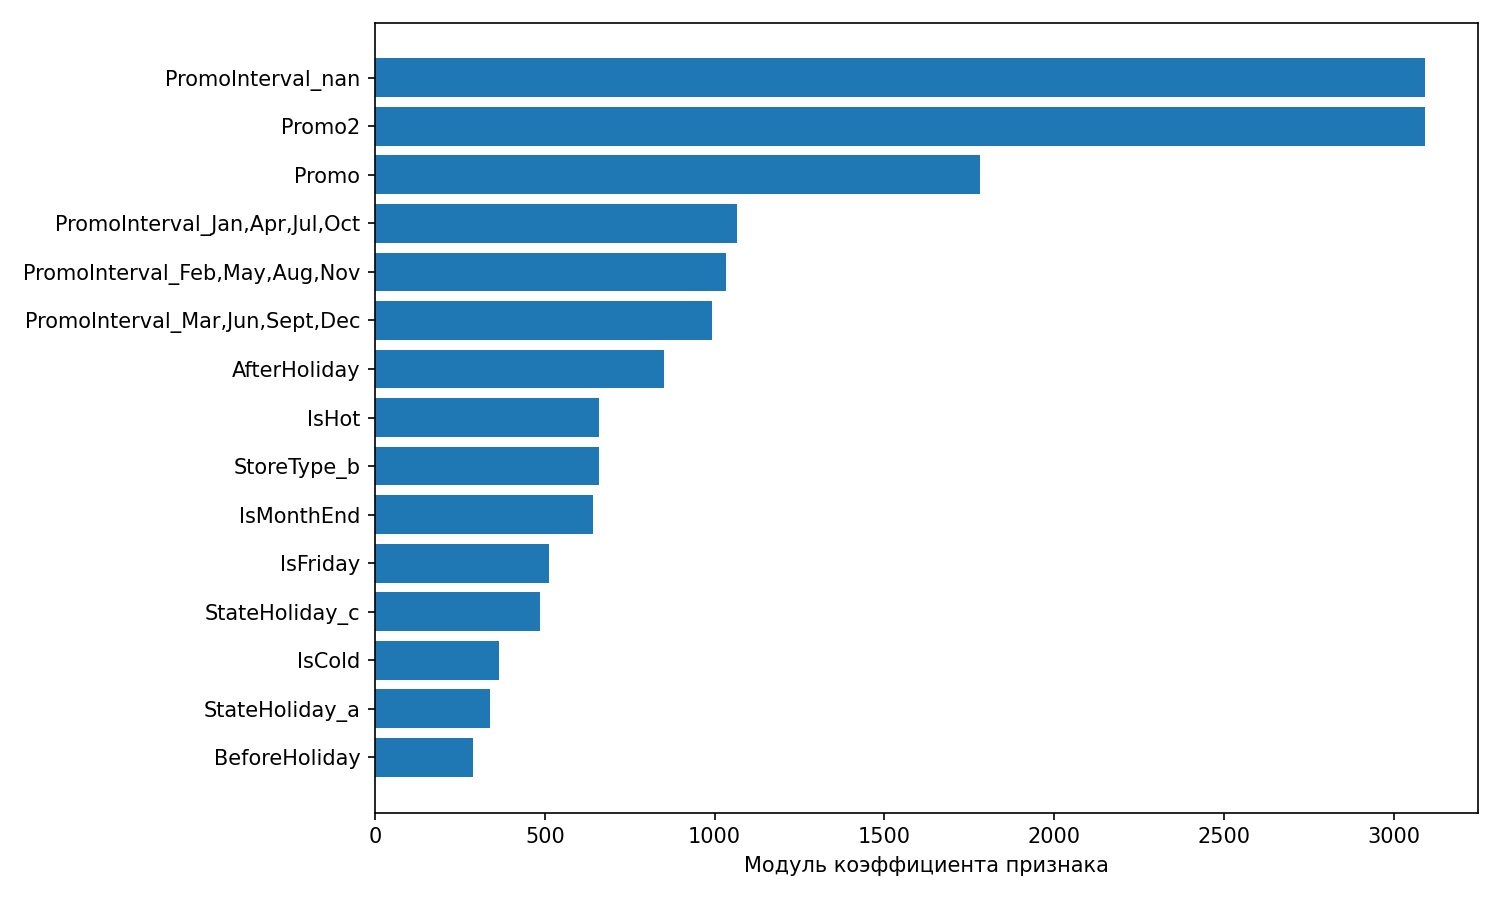
\includegraphics[width=0.9\linewidth]{importance_lr.png}
    \caption{Топ-15 признаков Linear Regression по модулю коэффициента}
    \label{fig:importance_lr}
\end{figure}

Для линейной регрессии анализ проводился на основе модулей коэффициентов модели. Наибольшие по модулю коэффициенты соответствуют признакам, связанным с промо-акциями: \texttt{PromoInterval\_nan}, \texttt{Promo2}, \texttt{Promo}, а также фиктивным признакам, кодирующим месячные интервалы участия магазина в промо-кампаниях \texttt{Promo2}. Кроме того, в число признаков с наибольшими по модулю коэффициентами вошли праздничные и календарные признаки: \texttt{AfterHoliday}, \texttt{BeforeHoliday}, \texttt{StateHoliday\_a}, \texttt{StateHoliday\_c}, \texttt{IsMonthEnd}, \texttt{IsFriday}.

Следует отметить, что интерпретация коэффициентов линейной регрессии имеет ряд ограничений. Абсолютная величина коэффициента зависит от масштаба соответствующего признака, а также от наличия корреляции между признаками. Поскольку признаки не приводились к единому масштабу, данный график не следует рассматривать как строгую оценку. Например, \texttt{Promo2} и \feat{PromoInterval_nan} содержательно связаны между собой, поэтому высокие значения их коэффициентов не следует трактовать как полностью независимый вклад каждого признака в прогноз целевой переменной. Тем не менее анализ коэффициентов позволяет выявить группы признаков, наиболее активно используемые линейной моделью.

\begin{figure}[H]
    \centering
    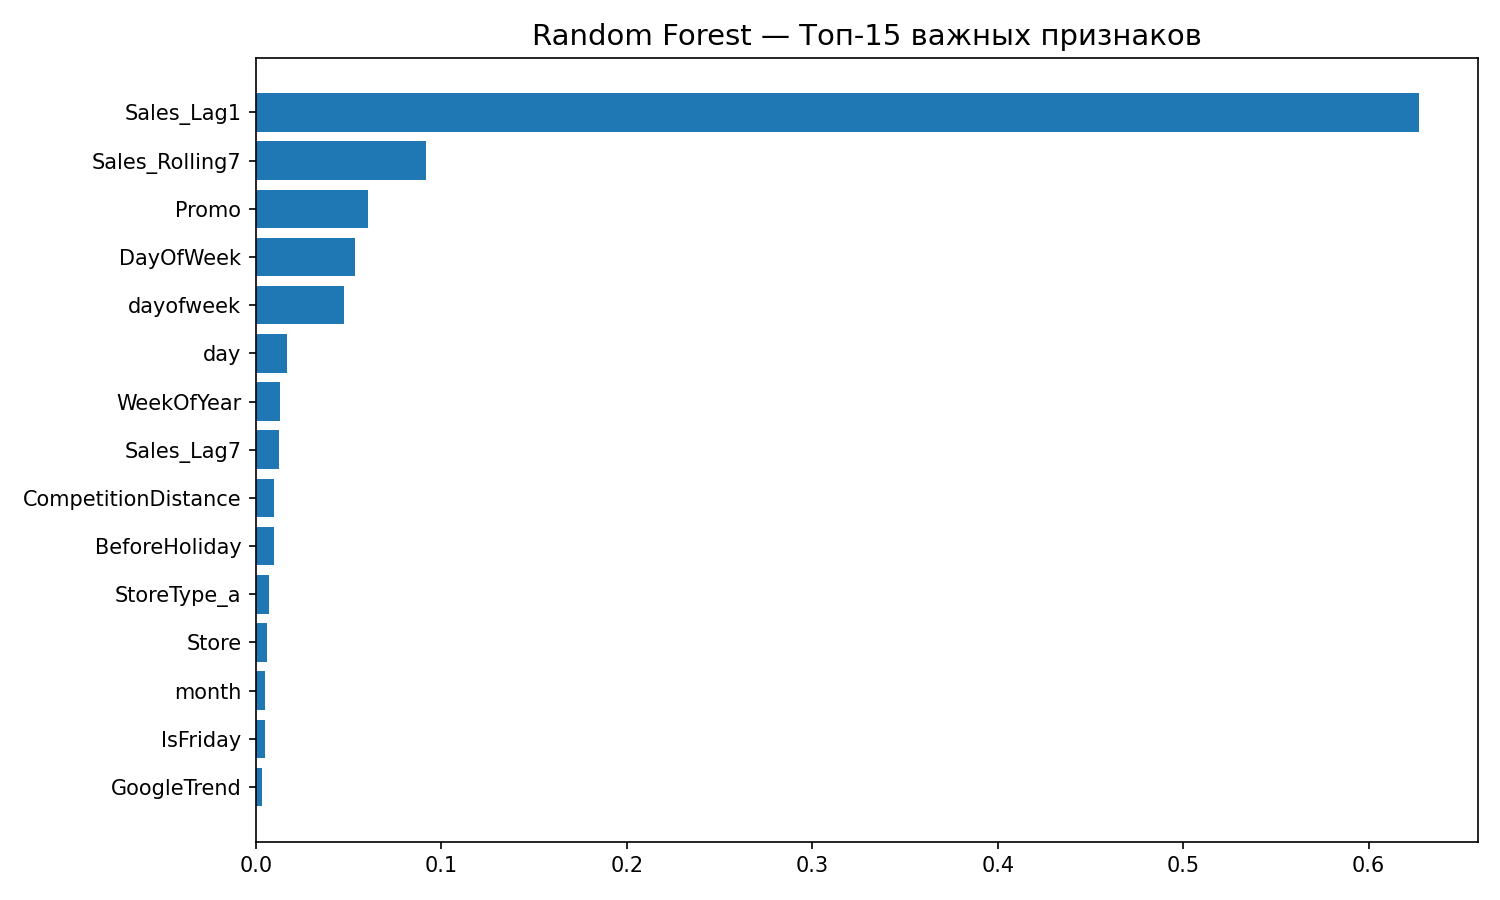
\includegraphics[width=0.8\linewidth]{importance_rf.png}
    \caption{Топ-15 важных признаков Random Forest}
    \label{fig:importance_rf}
\end{figure}

Для модели Random Forest важность признаков оценивалась на основе встроенной меры важности по уменьшению критерия разбиения (impurity-based feature importance), рассчитываемой по среднему уменьшению критерия MSE в деревьях ансамбля. Все важности в Random Forest нормируются так, что сумма важностей всех признаков равна 1. Наиболее важным для модели признаком оказался \texttt{Sales\_Lag1}. Его вклад существенно превышает вклад остальных признаков, что свидетельствует о сильной связи прогноза текущего наблюдения с уровнем продаж в предыдущем доступном наблюдении.

Следующими по важности для Random Forest являются признаки средней истории продаж за 7 предыдущих наблюдений, промоакции, дня недели, календарные признаки и недельный лаг продаж.

При интерпретации данной диаграммы важно учитывать, что встроенная мера важности может быть смещена в пользу числовых признаков и признаков с большим числом возможных разбиений \cite{strobl2007bias}. Более строгая проверка могла бы включать оценку важности признаков после их перемешивания на валидационной выборке, однако в данной работе она не проводилась.

\begin{figure}[H]
    \centering
    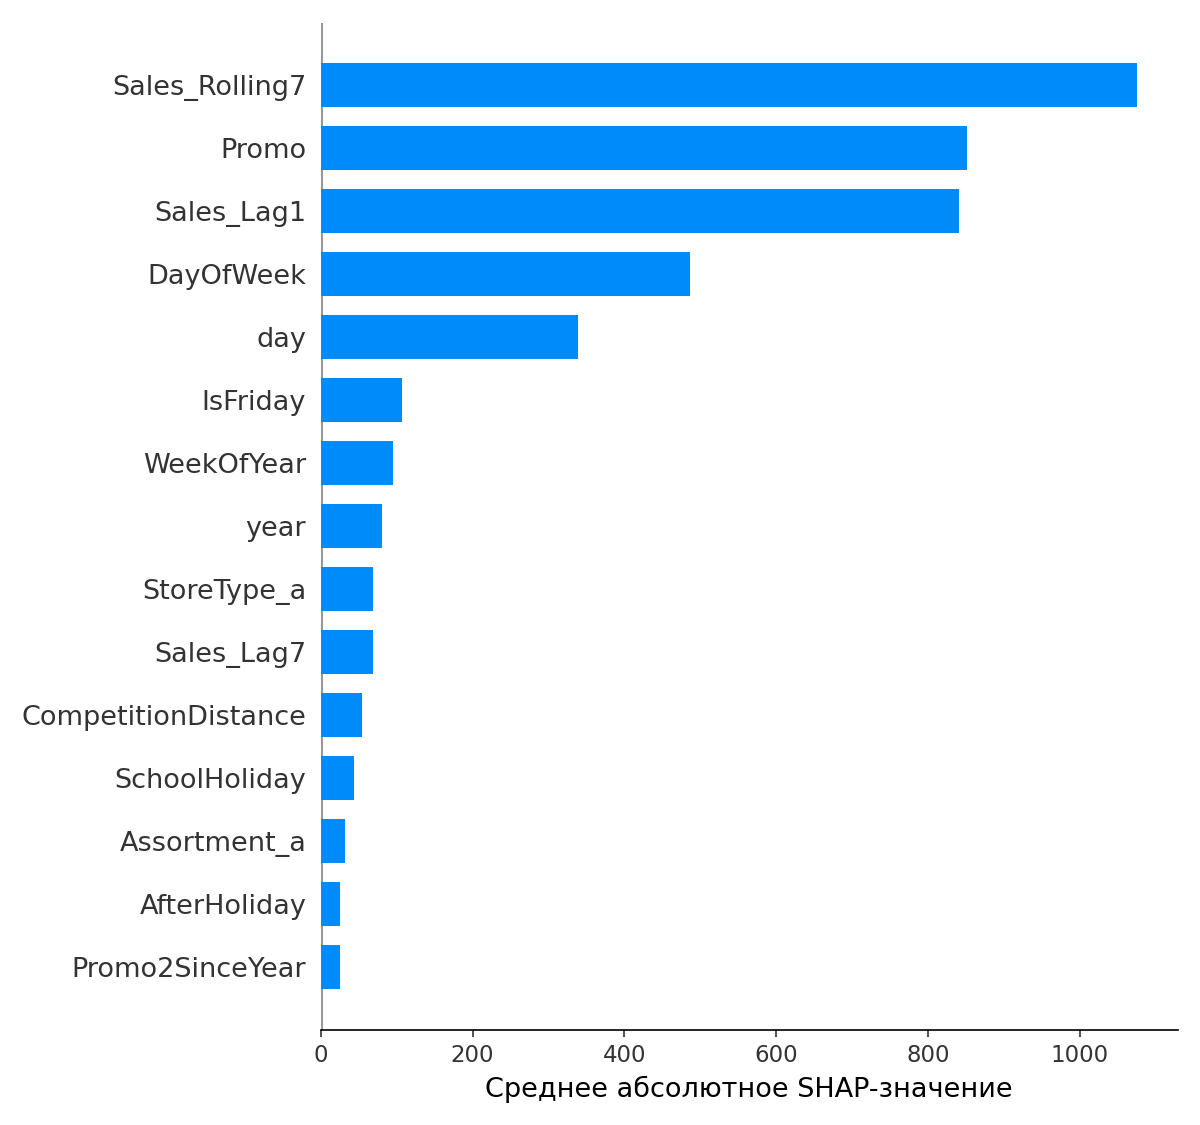
\includegraphics[width=0.9\linewidth]{shap_bar_holidays_lags.png}
    \caption{Средняя абсолютная важность признаков XGBoost по SHAP}
    \label{fig:shap_bar}
\end{figure}

Для модели XGBoost был применён SHAP-анализ. В отличие от встроенной в Random Forest меры важности признаков, SHAP-значения позволяют рассматривать не только средний вклад признака, но и направление этого вклада. Согласно графику средней абсолютной важности, наибольший вклад в прогноз XGBoost вносят признаки \texttt{Sales\_Rolling7}, \texttt{Promo}, \texttt{Sales\_Lag1}, \texttt{DayOfWeek}, \texttt{day}, \texttt{IsFriday}, \texttt{WeekOfYear} и \texttt{Sales\_Lag7}. Таким образом, XGBoost, как и Random Forest, в первую очередь использует информацию о продажах за предыдущие доступные наблюдения, промоакциях и календарном периоде.

\begin{figure}[H]
    \centering
    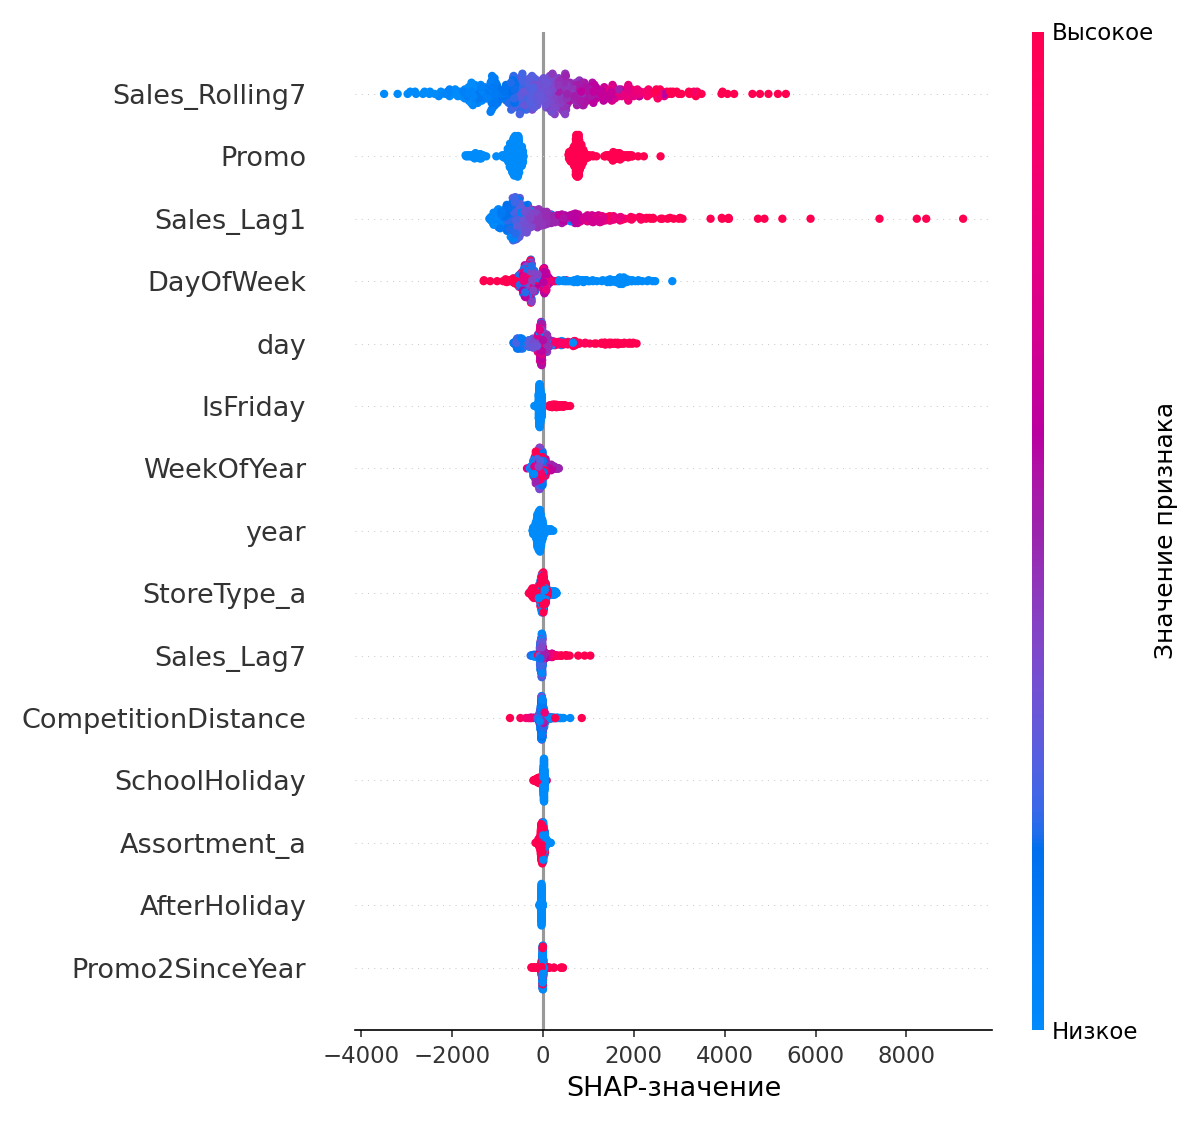
\includegraphics[width=0.9\linewidth]{shap_summary_holidays_lags.png}
    \caption{Направление вклада признаков в прогноз XGBoost}
    \label{fig:shap_summary}
\end{figure}

Summary-график SHAP дополнительно показывает характер вклада признаков в прогноз. Высокие значения \texttt{Sales\_Rolling7}, \texttt{Sales\_Lag1} и \texttt{Sales\_Lag7}, как правило, смещают прогноз продаж вверх, что подтверждает наличие инерционности продаж. Признак \texttt{Promo} также преимущественно даёт положительный вклад в прогноз, поскольку проведение промо-акций связано с ростом ожидаемых продаж. Для признака \texttt{DayOfWeek} различные значения дня недели могут как увеличивать, так и уменьшать прогноз, что указывает на различия в продажах между днями недели.

Сопоставление результатов для трёх моделей показывает, что наиболее информативными являются лаговые признаки продаж, признаки промоакций и календарные признаки. Внешние признаки, такие как погодные показатели и уровень безработицы, не вошли в число наиболее важных признаков для лучших древесных моделей. Это свидетельствует о том, что в рассматриваемой задаче их вклад в качество прогнозирования оказался ниже по сравнению с выше перечисленными признаками.

\section{Обсуждение}

\subsection{Анализ результатов экспериментов}

Главная закономерность, выявленная при сравнении вариантов признаков, состоит в определяющей роли лаговых признаков продаж. Для Random Forest переход от базового набора признаков к набору \texttt{lags} снизил RMSPE с \(0.2504\) до \(0.1461\), то есть примерно на \(41.6\%\). Лучший вариант Random Forest, \texttt{weather\_\_holidays\_\_lags}, дополнительно снизил RMSPE до \(0.1429\). Аналогичная картина наблюдается и для XGBoost: базовая модель получила RMSPE \(0.1930\), тогда как вариант \texttt{holidays\_\_lags} достиг RMSPE \(0.1439\).

Погодные признаки без лаговых признаков не дали устойчивого улучшения качества. Для Random Forest добавление только погодных признаков практически не изменило RMSPE относительно базового варианта: \(0.2504\) для \texttt{base} и \(0.2499\) для \texttt{weather}. Более того, комбинация \texttt{weather\_\_holidays} для Random Forest оказалась хуже базового варианта по RMSPE: \(0.2560\) против \(0.2504\). Для XGBoost погодные признаки улучшали качество относительно \texttt{base}, однако основной прирост всё равно был связан именно с добавлением лагов.

Признак Google Trends также не показал устойчивого положительного эффекта. Например, для Random Forest варианты \texttt{weather} и \texttt{weather\_\_google\_trends} дали практически одинаковые значения RMSPE, а для XGBoost добавление Google Trends к погодным признакам ухудшило RMSPE с \(0.1714\) до \(0.1743\). Возможное объяснение состоит в том, что агрегированный поисковый интерес слабо связан с ежедневными продажами конкретных магазинов или уже частично отражается через календарные и исторические признаки.

Ограниченный вклад внешних данных может быть связан с уровнем их агрегации. Погодные данные были присоединены по федеральной земле и дате, поэтому они не отражают точные погодные условия около каждого магазина. Показатель безработицы использовался на месячном уровне и поэтому слабо описывает ежедневные колебания продаж. Google Trends отражает региональный поисковый интерес по запросу \texttt{rossmann}, но такой интерес может быть связан с брендом в целом, а не с фактическим спросом в конкретном магазине в конкретный день.

Таким образом, исходная гипотеза о возможной полезности внешних признаков подтвердилась только частично. Отдельные комбинации с погодными и праздничными признаками улучшали качество, однако основной прирост был связан с лаговыми признаками.

В данном исследовании XGBoost не превзошёл Random Forest по значению RMSPE, несмотря на сильные позиции градиентного бустинга в задачах табличного машинного обучения. Вероятно, это связано с фиксированными гиперпараметрами и высокой ролью лаговых, промо- и календарных признаков. Поэтому результат следует трактовать только в рамках выбранного разбиения данных, набора признаков и настроек моделей.

Линейная регрессия показала заметно худшее качество по сравнению с древесными ансамблями: лучший вариант Linear Regression получил RMSPE \(0.2026\), тогда как лучшие Random Forest и XGBoost находились около \(0.143\). Это указывает на наличие нелинейных зависимостей между признаками и продажами.

\subsection{Интерпретация основных результатов}

Основным результатом работы является эмпирическая оценка вклада различных групп признаков в качество прогнозирования дневных продаж магазинов Rossmann. В отличие от простого сравнения нескольких моделей, в исследовании проведён перебор 48 вариантов набора признаков для трёх классов моделей: Linear Regression, Random Forest и XGBoost.

Основные результаты исследования можно сформулировать следующим образом:
\begin{itemize}
    \item установлено, что наибольший вклад в качество прогнозирования дают лаговые признаки продаж;
    \item показано, что внешние признаки без лаговых признаков дают ограниченный прирост качества и в ряде случаев не улучшают прогноз относительно базовых вариантов;
    \item выявлено, что в рамках заданных параметров и выбранного временного разбиения минимальное значение RMSPE было получено для Random Forest с набором признаков \texttt{weather\_\_holidays\_\_lags};
    \item показано, что XGBoost даёт близкое к Random Forest качество, однако в проведённом переборе при фиксированных гиперпараметрах Random Forest чаще занимал верхние позиции;
    \item установлено, что использование максимального количества признаков не гарантирует наилучшего качества прогноза.

\end{itemize}
\subsection{Практическая значимость}

Полученные результаты имеют практическое значение для задач операционного планирования в розничной торговле. Точный прогноз дневных продаж может использоваться для планирования товарных запасов, снижения риска дефицита товаров, оптимизации поставок и распределения персонала между магазинами. Кроме того, оценка важности признаков показывает, какие источники данных целесообразно учитывать в первую очередь при построении прикладной модели прогнозирования.

С практической точки зрения наиболее полезным результатом является вывод о высокой важности истории продаж, промоакций и календарных признаков. Это означает, что при ограниченных ресурсах на сбор внешних данных приоритет следует отдавать их корректному формированию. Внешние источники, такие как погода, Google Trends и уровень безработицы, следует добавлять только после проверки их вклада на валидационной выборке.

\subsection{Ограничения исследования и возможные улучшения}

Проведённое исследование имеет ряд ограничений, которые необходимо учитывать при интерпретации результатов.

\begin{itemize}
    \item Использовался один набор данных Rossmann Store Sales, поэтому выводы могут зависеть от специфики данной торговой сети и рассматриваемого периода.
    \item Для оценки качества применялось одно временное разбиение на обучающую и валидационную выборки, поэтому устойчивость различий между моделями не проверялась на нескольких периодах. Более строгая проверка могла бы включать последовательную временную валидацию на нескольких сдвигаемых периодах.
    \item Набор базовых прогнозов был расширен наивными лаговыми вариантами и средними продажами по магазину и дню недели. При этом более сложные статистические базовые модели, например экспоненциальное сглаживание или модели семейства ARIMA, в работе не рассматривались.
    \item Внешние признаки были агрегированы на уровне даты и региона, что могло сгладить локальные эффекты погоды и поискового интереса; показатель уровня безработицы использовался на месячном уровне. Кроме того, признак Google Trends имел недельную частоту и в текущей предобработке не распространялся на все дни соответствующей недели.
    \item В работе не моделировались возможные задержки публикации внешних данных. В таком случае можно было бы брать, например, последнее доступное значение на момент прогноза.
    \item Не проводился полный подбор гиперпараметров, из-за высокой вычислительной трудоёмкости и отсутствия цели в максимальной оптимизации каждой модели.
    \item Признак \texttt{Store} использовался как числовой, хотя содержательно он является категориальным. Кроме того, признаки \texttt{DayOfWeek} и \texttt{dayofweek} дублируют друг друга. В дальнейшем эти технические особенности предобработки следует устранить.
    \item Для Random Forest использовалась встроенная важность признаков, основанная на уменьшении критерия разбиения. Такая мера может быть смещена в пользу числовых признаков и признаков с большим числом возможных разбиений. Более строгая проверка могла бы включать важность по перемешиванию признаков (permutation importance) на валидационной выборке, однако это потребовало бы дополнительных вычислительных затрат и отдельного анализа коррелирующих признаков.
    \item В работе не рассматривались CatBoost, LightGBM и нейросетевые модели временных рядов, которые могут быть исследованы в дальнейшем.
    \item Для линейной регрессии ограничением является линейная зависимость фиктивных признаков. Это ограничение в меньшей степени относится к древесным моделям, таким как Random Forest и XGBoost, однако влияет на корректность интерпретации коэффициентов линейной модели.
\end{itemize}


\section{Заключение}

В результате проведённого исследования было установлено, что наибольший вклад в повышение качества прогнозирования дневных продаж вносят \textbf{лаговые признаки}, отражающие краткосрочную инерционность спроса. Это подтверждается тем, что все лучшие варианты моделей по метрике \(\mathrm{RMSPE}\) включали группу \texttt{lags}.

Минимальное значение RMSPE среди всех протестированных конфигураций было получено для модели Random Forest с набором признаков \feat{weather__holidays__lags}. Значение \(\mathrm{RMSPE}\) составило \(0.1429\), \(\mathrm{MAE}\) --- \(683\ \text{EUR}\), а коэффициент детерминации \(R^2\) --- \(0.8986\).

Исследовательская гипотеза подтвердилась частично. Внешние признаки не во всех конфигурациях улучшали качество прогнозирования, а основной вклад в снижение ошибки был связан с лаговыми признаками продаж. Поэтому включение внешних источников данных в модель требует предварительной эмпирической проверки на валидационной выборке.

Кроме того, результаты показали, что максимальное расширение набора признаков не гарантирует повышения качества прогнозирования. Более компактные наборы признаков, включающие лаги, праздничные и погодные признаки, оказались эффективнее некоторых расширенных комбинаций.

Таким образом, в рамках выбранного временного разбиения, фиксированных гиперпараметров и рассмотренных наборов признаков наиболее обоснованным кандидатом является Random Forest с набором признаков \feat{weather__holidays__lags}. Этот результат можно рассматривать как номинально лучший вариант внутри проведённого эксперимента, однако он не означает универсального превосходства Random Forest над XGBoost. Модели XGBoost показали близкое качество и могут быть дополнительно исследованы при более широком подборе гиперпараметров.

\begin{thebibliography}{14}

\bibitem{kaggle2015rossmann}
Rossmann Store Sales : dataset [Электронный ресурс] // Kaggle. --- 2015. ---
URL: \url{https://www.kaggle.com/c/rossmann-store-sales} (дата обращения:
15.05.2026).

\bibitem{fildes2022retail}
Fildes R., Ma S., Kolassa S. Retail forecasting: research and practice //
International Journal of Forecasting. --- 2022. --- Vol. 38, no. 4. ---
P. 1283--1318. --- DOI: 10.1016/j.ijforecast.2019.06.004.

\bibitem{makridakis2022m5}
Makridakis S., Spiliotis E., Assimakopoulos V. M5 accuracy competition:
results, findings, and conclusions // International Journal of Forecasting. ---
2022. --- Vol. 38, no. 4. --- P. 1346--1364. ---
DOI: 10.1016/j.ijforecast.2021.11.013.

\bibitem{ma2016demand}
Ma S., Fildes R., Huang T. Demand forecasting with high dimensional data: the
case of SKU retail sales forecasting with intra- and inter-category promotional
information // European Journal of Operational Research. --- 2016. ---
Vol. 249, no. 1. --- P. 245--257. --- DOI: 10.1016/j.ejor.2015.08.029.

\bibitem{rose2022weather}
Rose N., Dolega L. It's the weather: quantifying the impact of weather on
retail sales // Applied Spatial Analysis and Policy. --- 2022. --- Vol. 15,
no. 1. --- P. 189--214. --- DOI: 10.1007/s12061-021-09397-0.

\bibitem{choi2012predicting}
Choi H., Varian H. Predicting the present with Google Trends // The Economic
Record. --- 2012. --- Vol. 88, no. s1. --- P. 2--9. ---
DOI: 10.1111/j.1475-4932.2012.00809.x.

\bibitem{hyndman2021fpp}
Hyndman R. J., Athanasopoulos G. Forecasting: principles and practice
[Электронный ресурс]. --- 3rd ed. --- OTexts, 2021. ---
URL: \url{https://otexts.com/fpp3/} (дата обращения: 15.05.2026).

\bibitem{friedman2001greedy}
Friedman J. H. Greedy function approximation: a gradient boosting machine //
The Annals of Statistics. --- 2001. --- Vol. 29, no. 5. --- P. 1189--1232. ---
DOI: 10.1214/aos/1013203451.

\bibitem{chen2016xgboost}
Chen T., Guestrin C. XGBoost: a scalable tree boosting system // Proceedings
of the 22nd ACM SIGKDD International Conference on Knowledge Discovery and Data
Mining. --- 2016. --- P. 785--794. --- DOI: 10.1145/2939672.2939785.

\bibitem{breiman2001random}
Breiman L. Random forests // Machine Learning. --- 2001. --- Vol. 45. ---
P. 5--32. --- DOI: 10.1023/A:1010933404324.

\bibitem{openmeteo}
Historical Weather API [Электронный ресурс] // Open-Meteo. ---
URL: \url{https://open-meteo.com/en/docs/historical-weather-api} (дата
обращения: 15.05.2026).

\bibitem{googletrends}
Google Trends [Электронный ресурс] // Google. ---
URL: \url{https://trends.google.com/} (дата обращения: 15.05.2026).

\bibitem{fredunemployment}
Harmonized Unemployment Rate: All Persons for Germany [Электронный ресурс] //
Federal Reserve Bank of St. Louis. ---
URL: \url{https://fred.stlouisfed.org/series/LRHUTTTTDEM156S} (дата обращения:
15.05.2026).

\bibitem{strobl2007bias}
Strobl C., Boulesteix A.-L., Zeileis A., Hothorn T. Bias in random forest
variable importance measures: illustrations, sources and a solution //
BMC Bioinformatics. --- 2007. --- Vol. 8. --- Article 25. ---
DOI: 10.1186/1471-2105-8-25.

\end{thebibliography}

\end{document}
